% ---------------------------------------------------------------------------
% Author guideline and sample document for EG publication using LaTeX2e input
% D.Fellner, v1.12, Nov 01, 2006
\documentclass{egpubl}
\usepackage{hpg2010}

% --- for  Annual CONFERENCE
% \ConferenceSubmission % uncomment for Conference submission
% \ConferencePaper      % uncomment for (final) Conference Paper
% \STAR                 % uncomment for STAR contribution
% \Tutorial             % uncomment for Tutorial contribution
% \ShortPresentation    % uncomment for (final) Short Conference Presentation
%
% --- for  CGF Journal
% \JournalSubmission    % uncomment for submission to Computer Graphics Forum
% \JournalPaper         % uncomment for final version of Journal Paper
%
% --- for  EG Workshop Proceedings
%\WsSubmission    % uncomment for submission to EG Workshop
\WsPaper         % uncomment for final version of EG Workshop contribution
%
 \electronicVersion % can be used both for the printed and electronic version

% !! *please* don't change anything above
% !! unless you REALLY know what you are doing
% ------------------------------------------------------------------------

% for including postscript figures
% mind: package option 'draft' will replace PS figure by a filname within a frame
\ifpdf \usepackage[pdftex]{graphicx} \pdfcompresslevel=9
\else \usepackage[dvips]{graphicx} \fi

\PrintedOrElectronic

% prepare for electronic version of your document
\usepackage{t1enc,dfadobe}

\usepackage{egweblnk}
\usepackage{cite}

\usepackage{framed}
\usepackage[numbered]{algorithm}
\usepackage[noend]{algorithmic}
\usepackage{newalg}
\usepackage{subfigure}
\usepackage{graphics}
\usepackage{amsmath}
\usepackage{amssymb}
\usepackage{amsmath}

% For backwards compatibility to old LaTeX type font selection.
% Uncomment if your document adheres to LaTeX2e recommendations.
\let\rm=\rmfamily    \let\sf=\sffamily    \let\tt=\ttfamily
\let\it=\itshape     \let\sl=\slshape     \let\sc=\scshape
\let\bf=\bfseries

\newcommand{\leftbracket}{\left(}
\newcommand{\rightbracket}{\right)}

\newcommand{\leftcbracket}{\left\{}
\newcommand{\rightcbracket}{\right\}}

\newcommand{\leftvbracket}{\left|}
\newcommand{\rightvbracket}{\right|}

\newcommand{\leftsbracket}{\left[}
\newcommand{\rightsbracket}{\right]}

\newcommand{\boldx}{{\mathbf x}}
\newcommand{\boldn}{{\mathbf n}}
\newcommand{\boldv}{{\mathbf v}}
\newcommand{\boldy}{{\mathbf y}}

\newcommand{\phixt}{ \mathit{\phi} \leftbracket \boldx , t \rightbracket }
\newcommand{\phixtmdt}{ \mathit{\phi} \leftbracket \boldx , t - \Delta t \rightbracket }
\newcommand{\phixtmtdt}{ \mathit{\phi} \leftbracket \boldx , t - 2 \Delta t \rightbracket }

\newcommand{\conditionone}{ { \varsigma }_{1} \leftbracket \boldx , t \rightbracket }
\newcommand{\conditiontwo}{ { \varsigma }_{2} \leftbracket \boldx , t \rightbracket }

\newcommand{\ix}{I \leftbracket \boldx \rightbracket}

\newcommand{\nx}{ \eta \leftbracket \boldx \rightbracket }
\newcommand{\nv}{ \eta \leftbracket \boldv \rightbracket }
\newcommand{\nn}{ \eta \leftbracket \boldn \rightbracket }

\newcommand{\curvatureterm}{ \nabla \cdot \frac{\nabla \phixtmdt }{ \leftvbracket \nabla \phixtmdt \rightvbracket } }

\newcommand{\phiread}{ \phi^{read} }
\newcommand{\phiwrite}{ \phi^{write} }

\newcommand{\domainphi}{ \mbox{Domain} \leftbracket \phi \rightbracket }
\newcommand{\domainphiread}{ \mbox{Domain} \leftbracket \phiread \rightbracket }
\newcommand{\domainphiwrite}{ \mbox{Domain} \leftbracket \phiwrite \rightbracket }
\newcommand{\domainu}{ \mbox{Domain} \leftbracket U \rightbracket }

\newcommand{\qed}{\hfill \ensuremath{\Box}}

\floatstyle{boxed}
\newfloat{Listing}{h}

\newtheorem{cla}{Claim}
\newtheorem{lem}{Lemma}
\newtheorem{pro}{Proof}

% end of prologue

% ---------------------------------------------------------------------
% EG author guidelines plus sample file for EG publication using LaTeX2e input
% D.Fellner, v1.16, Jan 21, 2009


\title[A Work-Efficient GPU Algorithm for Level Set Segmentation]%
      {A Work-Efficient GPU Algorithm for Level Set Segmentation}

\author[Roberts, Packer, Sousa, Mitchell]
       {Mike Roberts, Jeff Packer, Mario Costa Sousa, Joseph Ross Mitchell
        \\
        University of Calgary, Canada
       }

% ------------------------------------------------------------------------

% if the Editors-in-Chief have given you the data, you may uncomment
% the following five lines and insert it here
%
% \volume{27}   % the volume in which the issue will be published;
% \issue{1}     % the issue number of the publication
% \pStartPage{1}      % set starting page


%-------------------------------------------------------------------------
\begin{document}

\maketitle

\begin{abstract}

We present a novel GPU level set segmentation algorithm that is both work-efficient and step-efficient. Our algorithm: (1) has linear work-complexity and logarithmic step-complexity, both of which depend only on the size of the active computational domain and do not depend on the size of the level set field; (2) limits the active computational domain to the minimal set of changing elements by examining both the temporal and spatial derivatives of the level set field; (3) tracks the active computational domain at the granularity of individual level set field elements instead of tiles without performance penalty; and (4) employs a novel parallel method for removing duplicate elements from unsorted data streams in a constant number of steps. We apply our algorithm to 3D medical images and we demonstrate that in typical clinical scenarios, our algorithm reduces the total number of processed level set field elements by $16 \times$ and is $14 \times$ faster than previous GPU algorithms with no reduction in segmentation accuracy.

\end{abstract}


%-------------------------------------------------------------------------
\section{Introduction}
\label{sec:introduction}

Identifying distinct regions in images -- a task known as \emph{segmentation} -- is an important task in computer vision~\cite{Osher-2003} and medical imaging~\cite{Shattuck-2009}. The level set method is a powerful and flexible numerical technique for image segmentation under challenging conditions~\cite{Whitaker-1994} since the segmentation process can depend on both intrinsic factors (e.g. the curvature of the segmented regions) and extrinsic factors (e.g. the intensity or texture of the image). Lefohn et al.~\cite{Lefohn-2003-MICCAI} and Cates et al.~\cite{Cates-2004} showed that level set segmentation methods can reduce the variability of difficult segmentation tasks in medical imaging. However the flexibility of the level set method has historically resulted in long computation times and therefore limited clinical utility.

In this paper we describe a new GPU level set segmentation algorithm that dramatically improves computational efficiency without affecting segmentation accuracy. Our new algorithm results from two distinct contributions:

\begin{enumerate}

    \item A method for limiting the active computational domain to the minimal set of changing elements by examining both the temporal and spatial derivatives of the level set field; and

    \item A work-efficient~\cite{Atallah-1998} and step-efficient~\cite{Nyland-2000} mapping of this method to manycore GPU architectures that avoids traversing the entire level set field after initialization and employs a novel method of removing duplicate elements from unsorted data streams in a constant number of steps.

\end{enumerate}

We describe our algorithm and demonstrate significant performance benefits over previous GPU algorithms~\cite{Lefohn-2003-MICCAI,Lefohn-2003-Vis,Cates-2004,Lefohn-2004}. In a series of controlled experiments using noisy magnetic resonance images (MRIs) generated from the BrainWeb Simulated Brain Database~\cite{BrainWeb-2010,Kwan-1996,Cocosco-1997,Collins-1998,Kwan-1999}, we demonstrate that our algorithm: (1) reduces the total number of processed level set field elements by $16 \times$ and and converges $14 \times$ faster than previous GPU algorithms; and (2) produces equally accurate segmentations to previous GPU algorithms with less than 0.2\% variability in all experiments. Our algorithm runs entirely on the GPU without requiring any additional data processing on the CPU, thereby enabling interactive 3D visualization and real-time control of the evolving level set surface.


%-------------------------------------------------------------------------
\section{Background and Previous Work}
\label{sec:backgroundAndPreviousWork}

\subsection{Level Set Segmentation}

The level set method for image segmentation~\cite{Whitaker-1994} embeds an implicitly represented seed surface within an image, and then iteratively deforms the surface to envelop the containing region-of-interest (ROI). Each implicitly defined point on the surface is deformed along a path normal to the local surface. Level set segmentation methods commonly use an application-specific speed function $ F \leftbracket \boldx , t \rightbracket $ to determine the local rate of surface motion, where $\boldx$ is a coordinate in the image and $t$ is the current time in the simulation. For a more comprehensive review of level set methods and their applications to image segmentation, we refer the reader to Sethian~\cite{Sethian-1999}, and Osher and Paragios~\cite{Osher-2003}.

In this paper we adopt the speed function proposed by Lefohn et al.~\cite{Lefohn-2003-MICCAI,Lefohn-2003-Vis,Lefohn-2004}. This function determines surface speed according to the local mean surface curvature and the local intensity of the image. By taking into account the level set surface's curvature, we encourage a smooth surface and prevent the surface from leaking into undesired areas across weak, incidental connections at ROI boundaries. For the scalar field $ \phixt : \mathfrak{R}^4 \mapsto \mathfrak{R} $, we define our level set surface as $ \leftcbracket \boldx \mid \phixt = 0 \rightcbracket $.

As proposed by Lefohn et al.~\cite{Lefohn-2003-MICCAI,Lefohn-2003-Vis,Lefohn-2004}, we define the data term of our speed function $D \leftbracket \boldx \rightbracket = \varepsilon - \leftbracket \leftvbracket \ix \rightvbracket - T \rightbracket $ to be a function of the image intensity $\ix$, the user-specified target intensity $T$ that will encourage maximal surface growth, and a user-specified intensity window parameter $\varepsilon $ within which the level set surface is encouraged to grow. If $\ix$ is between $T-\varepsilon $ and $T+\varepsilon $, then $D \leftbracket \boldx \rightbracket $ will encourage surface growth, otherwise $D \leftbracket \boldx \rightbracket $ will encourage surface contraction. We define the curvature term of our speed function as $ C \leftbracket \boldx , t \rightbracket = \curvatureterm $, where $ \curvatureterm $ is the local mean surface curvature of the level set field from the previous iteration.

We define our speed function as $ F \leftbracket \boldx , t \rightbracket = \alpha C \leftbracket \boldx , t \rightbracket + \leftbracket 1 - \alpha \rightbracket D \leftbracket \boldx \rightbracket $ where $\alpha \in \leftsbracket 0 , 1 \rightsbracket $ is a user-specified blending term that controls the relative influence of the curvature and data terms on the behavior of our speed function. For a detailed account of how this speed function can be implemented, we refer the reader to Lefohn et al.~\cite{Lefohn-2004}. We express the level set field update equation as follows.
\begin{equation}
    \phixt = \phixtmdt + \Delta t F \leftbracket \boldx , t \rightbracket \leftvbracket \nabla \phixtmdt \rightvbracket
\label{eq:1}
\end{equation}
Two distinct algorithms for efficiently solving Equation~\ref{eq:1} are directly relevant to our work: The GPU narrow band algorithm~\cite{Lefohn-2003-MICCAI,Lefohn-2003-Vis,Cates-2004,Lefohn-2004,Jeong-2009} and the sparse field algorithm~\cite{Whitaker-1998,Peng-1999}.


%-------------------------------------------------------------------------
\subsection{The GPU Narrow Band Algorithm}

The narrow band algorithm~\cite{Adalsteinsson-1995} only computes level set field updates inside a small region (i.e. a narrow band) of elements around the implicitly defined level set surface. This algorithm has been successfully ported to the GPU~\cite{Lefohn-2003-MICCAI,Lefohn-2003-Vis,Cates-2004,Lefohn-2004,Jeong-2009} by using various virtual memory paging schemes to map the irregular and dynamic narrow band onto a physically contiguous domain better suited for GPU computation. These virtual memory paging schemes partition the level set field into tiles and map each active tile (i.e. each tile containing elements in the narrow band) to a contiguous physical block of GPU memory. GPU narrow band algorithms only perform level set computations on active tiles. This significantly improves performance and saves a large amount of GPU memory because inactive virtual tiles do not need to be stored on the GPU. In turn, this allows for images larger than the size of available GPU memory to be segmented.

Until very recently, GPU narrow band algorithms~\cite{Lefohn-2003-MICCAI,Lefohn-2003-Vis,Cates-2004,Lefohn-2004} have maintained the narrow band by using parallel data reduction techniques on the GPU in cooperation with the CPU. The GPU generates a down-sampled memory image of active tiles which is subsequently downloaded by the CPU at the end of each iteration. The CPU is responsible for traversing the down-sampled image, determining the narrow band for the next iteration, and communicating this result back to the GPU. Since the CPU must sequentially traverse the down-sampled image when updating the narrow band, these algorithms have $O(n)$ work-complexity~\cite{Atallah-1998} and step-complexity~\cite{Nyland-2000} where $n$ is the size of the active computational domain. Moreover since the CPU work for each iteration cannot begin until the GPU work is finished and vice versa, these algorithms are limited by the communication latency between the GPU and CPU.

Developed in parallel with our own work, the GPU narrow band algorithm very recently described by Jeong et al.~\cite{Jeong-2009} avoids the communication latency inherent in previous GPU narrow band algorithms by traversing the domain of active tiles in parallel on the GPU. When a thread determines that a new tile should become part of the narrow band, the thread appends that tile to a list of active tiles stored in GPU memory. Since many threads are potentially appending to this list in parallel, Jeong et al. use GPU atomic memory operations to serialize access to the list. Therefore this system also has $O(n)$ work-complexity and step-complexity.

%-------------------------------------------------------------------------
\subsection{The Sparse Field Algorithm}

In contrast to the GPU narrow band algorithm, the sparse field algorithm~\cite{Whitaker-1998,Peng-1999} incrementally updates a linked list of active elements on the CPU during each iteration. Therefore this algorithm's work-complexity is $O(n)$. The sparse field algorithm also reduces its total amount of work by a constant factor by tracking the active computational domain at the granularity of individual elements instead of tiles. Historically the sparse field algorithm has been poorly suited to parallel implementation due to its reliance on linked lists. No parallel implementation of the sparse field algorithm currently exists in the literature. Therefore its step-complexity is equal to its work-complexity.

GPU narrow band systems~\cite{Lefohn-2003-MICCAI,Lefohn-2003-Vis,Cates-2004,Lefohn-2004,Jeong-2009} have historically outperformed optimized sequential sparse field systems. Nonetheless the GPU narrow band system we tested took over 100 seconds to converge on the white and grey matter in a ${256}^3$ MRI of a human head on a state-of-the-art GPU. This limitation constrains clinical applications and motivates our work-efficient algorithm, which leverages ideas from both the GPU narrow band algorithm and the sparse field algorithm. We begin the presentation of our algorithm by describing our novel method for tracking the active computational domain.


%*******************************************************************************
% FIGURE 1
\begin{figure*}[t]
\centering
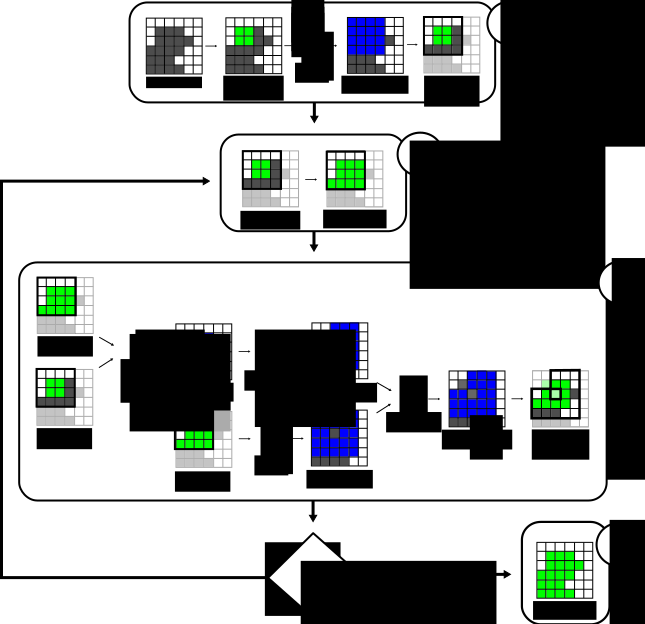
\includegraphics[width=6.0in]{figures/Algorithm.pdf}
\caption{Our algorithm for tracking the active computational domain. Image data is shown in grey, currently segmented regions are shown in green, and intermediate results for computing the active computational domain are shown in blue. The active computational domain is outlined in black, and inactive elements are shown as partially transparent. The user places a seed to initialize the level set field and the initial active computational domain is determined according to the spatial derivatives of the level set field (a). During each iteration the level set field is updated at all active elements (b). The new active computational domain is computed according to the temporal and spatial derivatives of the level set field (c). If the new active computational domain is empty (d) then our segmentation has globally converged (e). Otherwise we go to (b). }
\label{fig:1}
\end{figure*}
%*******************************************************************************


%-------------------------------------------------------------------------
\section{A Temporally Coherent Active Computational Domain}
\label{sec:aTemporallyCoherentActiveComputationalDomain}

The narrow band and sparse field algorithms described in the previous section avoid unnecessary computation by only updating field elements near the level set surface. We make the observation that even computations near the level set surface can be avoided in regions where the level set field has locally converged. This observation motivates our method of tracking the active computational domain according to both the temporal and spatial derivatives of the level set field.

We define the minimal set of active coordinates at time $t$ as $A \leftbracket t \rightbracket = \leftcbracket \boldx \mid \phixt \ne \phixtmdt \rightcbracket $. From Equation~\ref{eq:1} we derive two conditions, each of which is sufficient to imply that $ \boldx  \notin A \leftbracket t \rightbracket $. Both of these conditions are independent of our speed function and could therefore be applied to a variety of level set simulations.

The first condition ${ \varsigma }_{1}$ follows directly from Equation~\ref{eq:1} and can be expressed as follows: $ \conditionone \equiv \leftvbracket \nabla \phixtmdt \rightvbracket = 0 $. We note that ${ \varsigma }_{1}$ is described by Lefohn et al.~\cite{Lefohn-2003-Vis,Lefohn-2004}.

The second condition ${ \varsigma }_{2}$ requires a more detailed discussion. We define the set $ \nx $ as the set of all coordinates in the immediate neighborhood of $ \boldx $ (including $  \boldx $ itself). We observe that if $ \phixtmdt = \phixtmtdt $, then $ \frac{ \Delta \phi \leftbracket \boldx \rightbracket }{ \Delta t } = 0 $. In other words $ \phi $ is in a state of temporal equilibrium at $ \boldx $. Assuming the speed function is defined locally, the only event that could potentially disrupt this state of temporal equilibrium at $ \boldx $ is if $ \phi \leftbracket \boldn \rightbracket $ changes for some neighbor $ \boldn \in \nx $. If the level set field is in a state of temporal equilibrium in the neighborhood around $ \boldx $ at time $ t - 2 \Delta t $, then $ \boldx $ will continue to be in a state of temporal equilibrium at time $ t - \Delta t $. This leads to the following expression for ${ \varsigma }_{2}$: $ \conditiontwo \equiv { \forall }_{ \boldn \in \nx } : \phi \leftbracket \boldn , t - \Delta t \rightbracket = \phi \leftbracket \boldn , t - 2 \Delta t \rightbracket $.

We include a more formal derivation of ${ \varsigma }_{2}$ in Appendix~\ref{app:1}. For the logical \emph{not} operator $\lnot$ we formally express our active set as follows:
\begin{equation}
A \leftbracket t \rightbracket = 
\begin{cases} 
    \domainphi                                                                                                                      & t = 0        \\
    \leftcbracket \boldx \mid \lnot \conditionone \rightcbracket                                                                    & t = \Delta t \\
    \leftcbracket \boldx \mid \lnot \conditionone \rightcbracket \cap \leftcbracket \boldx \mid \lnot \conditiontwo \rightcbracket  & t > \Delta t \\
\end{cases}
\label{eq:4}
\end{equation}
%We note that ${ \varsigma }_1 $ appears in some form in existing literature~\cite{Jeong-2009,Lefohn-2003-MICCAI,Lefohn-2003-Vis,Cates-2004,Lefohn-2004}. As far as we know ${ \varsigma }_2 $ is a novel contribution to the literature.
A diagram describing our method of tracking the active computational domain is shown in Figure~\ref{fig:1}.


\begin{Listing}[t]
    \caption{Initializing the level set field to the signed and clamped distance transform relative to a user-specified seed sphere with the center $\mathbf{c}$ and the radius $r$. \label{pseudo:1} }
    \begin{algorithmic}[1]
        \FORALL { coordinates $\boldx \in \domainphi$ in parallel } 
            \STATE { $ \phiread_{\boldx} \gets \mbox{clamp} \leftbracket \| \boldx - \mathbf{c} \| - r \rightbracket $  }
            \STATE { $ \phiwrite_{\boldx} \gets \mbox{clamp} \leftbracket \| \boldx - \mathbf{c} \| - r \rightbracket $  }
        \ENDFOR
    \end{algorithmic}
\end{Listing}


%-------------------------------------------------------------------------
\section{A Work-Efficient Parallel Algorithm}
\label{sec:aWorkEfficientParallelAlgorithm}

We want to track the active computational domain and perform updates on the level set field in a way that is both work-efficient and step-efficient. In other words we want a parallel algorithm with work-complexity and step-complexity of at most $O(n)$. This upper bound on work-complexity and step-complexity motivates the algorithm described in this section. A high level overview of our algorithm is as follows:

\begin{enumerate}

    \item Initialize the level set field and generate a dense list of active coordinates.

    \item Update the level set field at all active coordinates.

    \item Generate new active coordinates. During this step generating duplicate active coordinates is permitted.

    \item Remove all duplicate active coordinates generated in (3).

    \item Compact all the unique new active coordinates from (4) into a new dense list.

    \item If there are no active coordinates in the new dense list, the segmentation has globally converged. Otherwise go to (2).

\end{enumerate}


%-------------------------------------------------------------------------
\subsection{Assumptions}
\label{subsec:assumptions}

We assume $ \phi $ is 3D and the voxels in $ \phi $ are 6-connected. Therefore it is guaranteed that for all voxels $ \boldx \in \domainphi $, the set $ \nx $ contains at most seven elements: the 6-connected neighbors of $ \boldx $ and $ \boldx $ itself. We define the set $ E = \leftcbracket \leftbracket 0,0,0 \rightbracket , \leftbracket \pm 1,0,0 \rightbracket , \leftbracket 0,\pm 1,0 \rightbracket , \leftbracket 0,0,\pm 1 \rightbracket \rightcbracket $ as the set of offset vectors from a voxel to its 6-connected neighbors.


%-------------------------------------------------------------------------
\subsection{Data Structures and Notation}
\label{subsec:dataStructuresAndNotation}

Our algorithm requires three 3D buffers: $\phiwrite$ and $\phiread$ to store the current and previous level set field respectively; and $U$ to use as a scratchpad. Our algorithm also requires eight 1D buffers: $V$ to store the current dense list of active coordinates; and $B^{ \leftbracket 0,0,0 \rightbracket }$, $B^{ \leftbracket \pm 1,0,0 \rightbracket }$, $B^{ \leftbracket 0, \pm 1,0 \rightbracket }$, and $B^{ \leftbracket 0,0, \pm 1 \rightbracket }$ to use as auxiliary buffers when generating new active coordinates. The size of each buffer is equal to the size of the entire level set field. All buffers are initially filled with null values.

In our implementation the data type of $\phiwrite$ and $\phiread$ is 32-bit floating point and the data type of all other buffers is 32-bit integer. To maximize memory efficiency when storing 3D level set field coordinates in these integer buffers, we pack the $x$, $y$, and $z$ components of each 3D coordinate into 11, 11, and 10 bits respectively. However if the level set field contains more than $2048 \times 2048 \times 1024 = 2^{32}$ elements, the data type of each integer buffer must be expanded such that the largest possible level set field coordinate can fit into a single element.

We use a subscript notation to refer to individual buffer elements. For example $V_i$ refers to the $i^{th}$ element of $V$; $V_{j \ldots k }$ refers to the range of elements in $V$ from $V_j$ to $V_k$; and $U_{\boldx}$ refers to the element of $U$ with the 3D coordinates $\boldx$.

%We use $V$ to store the current set of active coordinates. We use $\phiread$ and $\phiwrite$ to read from and write to the level set field in a double-buffered fashion. We use $ B^{ \leftbracket 0,0,0 \rightbracket }$, $B^{ \leftbracket 0,0, \pm 1 \rightbracket }$, $B^{ \leftbracket 0, \pm 1,0 \rightbracket }$, and $B^{ \leftbracket \pm 1,0,0 \rightbracket }$ as auxiliary buffers to store intermediate output as we're generating new active coordinates. Finally we use $U$ as a scratchpad buffer. All buffers are initially filled with null values.


%-------------------------------------------------------------------------
\subsection{Initialization}
\label{subsec:initialization}

We initialize in parallel every coordinate in $\phiread$ and $\phiwrite$ according to a user-specified seed region as shown in Listing~\ref{pseudo:1}. For more details on this initialization step we refer the reader to Lefohn et al.~\cite{Lefohn-2004}.

We then generate a densely packed buffer of active coordinates $V$ based on the contents of $\phiread$ as shown in Listing~\ref{pseudo:2}. We test every coordinate of $\phiread$ in parallel to determine which ones are active. If a coordinate is deemed active according to Equation~\ref{eq:4}, we write that coordinate to our 3D scratchpad $U$ using the coordinate itself as the 3D array index. We compact $U$ in parallel to produce $V$. We set the initial size of the active computational domain $n$ to be the number of coordinates that were compacted into $V$. For more details on this buffer compacting operation we refer the reader to Harris et al.~\cite{Harris-2007} and Sengupta et al.~\cite{Sengupta-2007,Sengupta-2008}. We note that since $U$ contains either a unique value or null at all coordinates, it is guaranteed that there are no duplicate coordinates in $V_{0 \ldots n$. At this point our algorithm has been fully initialized. We avoid traversing the entire level set field for the remainder of our algorithm.


%*******************************************************************************
% FIGURE 2
%\begin{figure}[t]
%\centering
%\includegraphics[width=3.0in]{figs/fig2.png}
%\caption{Initializing our list of active coordinates in parallel. We initialize in parallel a scratchpad buffer with active coordinates using the coordinates themselves as array indices. We then interpret the scratchpad buffer as one-dimensional and compact it in parallel to produce a densely packed buffer of active coordinates.}
%\label{fig:2}
%\end{figure}
%*******************************************************************************


\begin{Listing}[t]
    \caption{Initializing the list of active coordinates. The spatial derivative of the level set field is tested on line 5. \label{pseudo:2} }
    \begin{algorithmic}[1]
        \FORALL { coordinates $\boldx \in \domainphi$ in parallel }
            \STATE { $ g \gets \mbox{false} $ }
            \FORALL { coordinates $\boldn \in \nx$ }
                \IF { \textbf{not } $ g $ }
                    \IF { $ \phiread_{\boldx} \neq \phiread_{\boldn} $  }
                        \STATE { $ g \gets \mbox{true} $ }
                    \ENDIF    
                \ENDIF
            \ENDFOR
            \IF { $ g $ }
                \STATE { $ U_{\boldx} \gets \boldx $  }
            \ENDIF           
        \ENDFOR
        \STATE { $ V \gets \mbox{\textbf{compact}} \leftbracket U \rightbracket $  }
    \end{algorithmic}
\end{Listing}


\begin{Listing}[t]
    \caption{Updating the level set field according to Equation~\ref{eq:1} and clearing the scratchpad at all active coordinates. $n$ is the current size of the active computational domain. \label{pseudo:3} }
    \begin{algorithmic}[1]
        \FORALL { coordinates $\boldv \in V_{0 \ldots n}$ in parallel }
            \STATE { $ \phiwrite_{\boldv} \gets \phiread_{\boldv} + \Delta t F \leftbracket \boldv , t \rightbracket \ \leftvbracket \nabla \phiread_{\boldv} \rightvbracket $ }        
            \STATE { $ U_{\boldv} \gets \mbox{null} $  }                
        \ENDFOR
        \STATE { $ \mbox{\textbf{swap}} \leftbracket \phiread, \phiwrite \rightbracket $  }        
    \end{algorithmic}
\end{Listing}


%-------------------------------------------------------------------------
\subsection{Updating the Level Set Field}
\label{subsec:updatingTheLevelSetField}

During each iteration we update $\phiwrite$ and clear $U$ at all active coordinates as shown in Listing~\ref{pseudo:3}. This is guaranteed to completely clear $U$ because the only non-null values in $U$ are at active coordinates, each of which was previously compacted into $V$. At this point we are finished updating the level set field for this iteration, so we swap references to $\phiread$ and $\phiwrite$.


%-------------------------------------------------------------------------
\subsection{Generating New Active Coordinates}
\label{subsec:generatingNewActiveCoordinates}

We traverse our current list of active coordinates in parallel and test for new active coordinates according to Equation~\ref{eq:4}. We describe this process in Listing~\ref{pseudo:4} and Figure~\ref{fig:3}. We test $ { \varsigma }_{1} $ and $ { \varsigma }_{2} $ for the next iteration by examining $ \phiread = \phi \leftbracket t \rightbracket $ and $ \phiwrite = \phi \leftbracket t - \Delta t \rightbracket$. We note that at the end of this step, the seven auxiliary buffers may contain duplicate coordinates when taken collectively. This is because each thread tests a local neighborhood of coordinates and some coordinates may be tested repeatedly by different threads.



\begin{Listing}[t]
    \caption{Generating new active coordinates. The temporal and spatial derivatives of the level set field are tested on line 5. $n$ is the current size of the active computational domain. \label{pseudo:4} }
    \begin{algorithmic}[1]
        \FOR { $h \gets 0$ to $n$ in parallel }
            \STATE { $\boldv \gets V_h$ } 
            \STATE { $g \gets \mbox{false}$ }
            \FORALL { coordinates $\boldn \in \nv$ }
                \IF { $ \phiread_{\boldn} \neq \phiwrite_{\boldn} $ \textbf{ and } $ \phiread_{\boldn} \neq \phiread_{\boldv} $ }
                    \STATE { $g \gets \mbox{true}$ }
                    \STATE { $\mathbf{e} \gets \boldn - \boldv$ }
                    \STATE { $B^{\mathbf{e}}_{h} \gets \boldn $ }
                \ENDIF
            \ENDFOR
            \IF { $g$ }
                \STATE { $B^{ \leftbracket 0,0,0 \rightbracket }_{h} \gets \boldv $ }
            \ENDIF                    
        \ENDFOR
    \end{algorithmic}
\end{Listing}


%*******************************************************************************
% FIGURE 3
\begin{figure}[t]
\centering
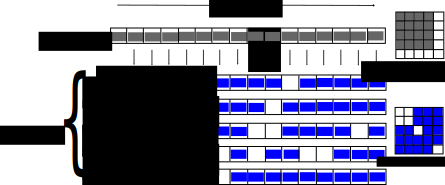
\includegraphics[width=3.0in]{figures/NewActive.pdf}
\caption{Generating new active coordinates. There may be duplicate coordinates in the auxiliary buffers when taken collectively. All duplicate coordinates must subsequently be removed (see Figure~\ref{fig:4}).}
\label{fig:3}
\end{figure}
%*******************************************************************************


%Since each new active coordinate is the 6-connected neighbor of some old active coordinate, and all 6-connected neighbors of all old active coordinates are tested by at least one thread, it is guaranteed that all new active coordinates are contained in at least one of the seven auxiliary buffers.

%Some thread $p$ may deem a coordinate $\mathbf{r}$ to be active. For the thread $p$ suppose that $\mathbf{r}-\mathbf{v}_p = \leftbracket 0,0,1 \rightbracket$ and therefore thread $p$ writes $\mathbf{r}$ to the auxiliary buffer $B^{ \leftbracket 0,0,1 \rightbracket }$. Some different thread $q$ may also deem the same coordinate $\mathbf{r}$ to be active. For the thread $q$ suppose that $\mathbf{r} - \mathbf{v}_q = \leftbracket 1,0,0 \rightbracket $ and therefore thread $q$ writes $\mathbf{r}$ to the auxiliary buffer $B^{ \leftbracket 1,0,0 \rightbracket }$. In this case $\mathbf{r}$ appears in both $B^{ \leftbracket 0,0,1 \rightbracket }$ and $B^{ \leftbracket 1,0,0 \rightbracket }$.

%-------------------------------------------------------------------------
\subsection{Removing Duplicate Active Coordinates}
\label{subsec:removingDuplicateActiveCoordinates}

We make the observation that although there may be duplicate coordinates in the seven auxiliary buffers taken collectively, it is guaranteed that there are no duplicate coordinates in each of the seven auxiliary buffers taken individually. This is because there are no duplicate coordinates in $V_{0 \ldots n}$ and for all offset vectors $\mathbf{e} \in E$, either $B^{\mathbf{e}}_{i} = V_i + \mathbf{e} $ or ${B^{\mathbf{e}}_i = \mbox{null}$ for all array indices $i$ where $0 \leq i \leq n$.

Based on the guarantee in the previous paragraph, we are able to remove all duplicate coordinates in seven passes without requiring any additional sorting or synchronization primitives. We describe this process in Listing~\ref{pseudo:5} and Figure~\ref{fig:4}.


\begin{Listing}[t]
    \caption{Generating a new dense list of unique active coordinates without sorting the auxiliary buffers. $n$ is the current size of the active computational domain. \label{pseudo:5} }
    \begin{algorithmic}[1]
        \STATE { $ E' \gets E - \leftcbracket \leftbracket 0,0,0 \rightbracket , \leftbracket 0,0,1 \rightbracket \rightcbracket $ }
        \FORALL { coordinates $\mathbf{b} \in B^{ \leftbracket 0,0,0 \rightbracket }_{0 \ldots n}$ in parallel }
            \IF { $ \mathbf{b} \neq \mbox{null}$ }
                \STATE { $ U_{\mathbf{b}} \gets \mbox{tagged}$ }
            \ENDIF
        \ENDFOR                        
        \FORALL { offset vectors $\mathbf{e} \in E' $ } 
            \FOR { $h \gets 0$ to $n$ in parallel }
                \STATE { $\mathbf{b} \gets B^{\mathbf{e}}_{h}$ }            
                \IF { $ \mathbf{b} \neq \mbox{null}$ }
                    \IF { $ U_{\mathbf{b}} = \mbox{tagged} $ }
                        \STATE { $B^{\mathbf{e}}_{h} \gets \mbox{null}$ }
                    \ELSE
                        \STATE { $U_{\mathbf{b}} \gets \mbox{tagged} $ }
                    \ENDIF                                            
                \ENDIF
            \ENDFOR
        \ENDFOR
        \FOR { $h \gets 0$ to $n$ in parallel }
            \STATE { $\mathbf{b} \gets B^{ \leftbracket 0,0,1 \rightbracket }_{h} $ }       
            \IF { $ \mathbf{b} \neq \mbox{null}$ \textbf{ and } $ U_{\mathbf{b}} = \mbox{tagged} $ }
                \STATE { $B^{ \leftbracket 0,0,1 \rightbracket }_{h} \gets \mbox{null}$ }
            \ENDIF
        \ENDFOR                        
        \STATE { $V \gets \mbox{\textbf{compact}} \leftbracket
            B^{ \leftbracket 0,0,0 \rightbracket }_{0 \ldots n},
            B^{ \leftbracket \pm 1, 0, 0 \rightbracket }_{0 \ldots n},
            B^{ \leftbracket 0, \pm 1, 0 \rightbracket }_{0 \ldots n},
            B^{ \leftbracket 0, 0, \pm 1 \rightbracket }_{0 \ldots n} \rightbracket$ }       
    \end{algorithmic}
\end{Listing}


%*******************************************************************************
% FIGURE 4
\begin{figure}[t]
\centering
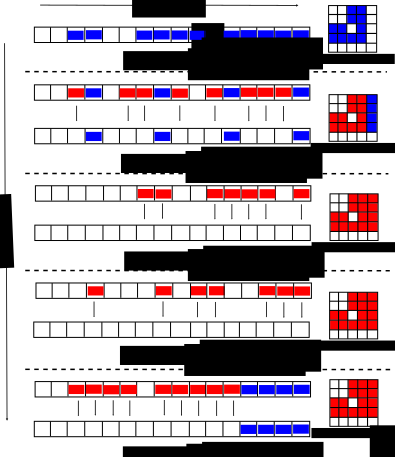
\includegraphics[width=3.0in]{figures/RemoveDuplicates-Alt.pdf}
\caption{Removing duplicate coordinates from the auxiliary buffers in parallel without sorting. Coordinates that have not been previously tagged in the scratchpad buffer are shown in blue. Coordinates that have been previously tagged in the scratchpad buffer are shown in red, and are removed from their containing auxiliary buffer. This process is free of race conditions because each step examines one auxiliary buffer and there are no duplicate coordinates within each auxiliary buffer.}
\label{fig:4}
\end{figure}
%*******************************************************************************


%-------------------------------------------------------------------------
\subsection{Compacting the New Active Coordinates}
\label{subsec:compactingTheNewActiveCoordinates} 

We compact the seven auxiliary buffers in parallel to produce a new dense list of active coordinates and store the result in $V$ as shown in Listing~\ref{pseudo:5}. Since we only ever write to the first $n$ elements of each auxiliary buffer, we only need to compact $7n$ elements in total, rather than compacting the total size of each buffer. In order to further improve the efficiency of this buffer compacting step, we allocate the auxiliary buffers dynamically at the beginning of each iteration by partitioning a larger pre-allocated buffer.

After compacting the seven auxiliary buffers, we check if any new active coordinates were compacted into $V$. If so, we clear $B^{\mathbf{e}}_{0 \ldots n}$ for all offset vectors $\mathbf{e} \in E$, update $n$ to be the number of new active coordinates that were compacted into $V$, and go to the step described in section~\ref{subsec:updatingTheLevelSetField}. Otherwise our algorithm has globally converged on the segmented region contained in $\phiread$.


%-------------------------------------------------------------------------
\subsection{Memory Efficiency}
\label{subsec:memoryEfficiency}

All memory accesses to the 1D buffers $V$, $B^{ \leftbracket 0,0,0 \rightbracket }$, $B^{ \leftbracket \pm 1, 0, 0 \rightbracket }$, $B^{ \leftbracket 0, \pm 1, 0 \rightbracket }$, and $B^{ \leftbracket 0, 0, \pm 1 \rightbracket }$ are fully coalesced. These buffers are always accessed via a unique thread index such that neighboring threads always access neighboring locations in memory.

In general none of the memory accesses to the 3D buffers $\phiread$, $\phiwrite$, and $U$ can be coalesced. After initialization these buffers are always accessed at sparse active coordinates which are not guaranteed to be neighboring for neighboring threads. Therefore it is not clear how to take advantage of GPU shared memory as a programmer-managed cache for level set computations using our algorithm. For this reason our implementation does not use GPU shared memory.

However since there is some spatial locality in the active computational domain, it is probable but not guaranteed that nearby active coordinates in $V$ are nearby in 3D space. We leverage this spatial locality by reading from our 3D buffers via the hardware-managed texture cache. To improve multi-dimensional cache coherence, we use a simple swizzled memory layout as described by Engel et al~\cite{Engel2006}.


%*******************************************************************************
% FIGURE 6
\begin{figure}[t]
\centering
\subfigure[ the aorta and kidneys in a $256 \times 256 \times 272$ abdominal CT image -- total computation time 16 seconds ]{
\includegraphics[width=3.0in]{figures/Aorta-3D.png}
\label{fig:aorta}
}
\subfigure[ the cortical bone and trabecular bone in a $288 \times 352 \times 112$ wrist CT image -- total computation time 12 seconds ]{
\includegraphics[width=3.0in]{figures/Bone-3D.png}
\label{fig:bone}
}
\caption{ Segmentation results from our system. }
\label{fig:qualitative}
\end{figure}
%*******************************************************************************

%*******************************************************************************
% FIGURE 6
\begin{figure}[t]
\centering
\includegraphics[width=3.0in]{figures/Brainweb-3D-Composite-Offset.png}
\caption{ The progression of our algorithm while segmenting the white and grey matter in a $256^3$ head MRI with a signal-to-noise ratio of 11 -- total computation time 7 seconds. }
\label{fig:brainweb3d}
\end{figure}
%*******************************************************************************


%-------------------------------------------------------------------------
\section{Evaluation}
\label{sec:evaluation}


%-------------------------------------------------------------------------
\subsection{Algorithmic Complexity}
\label{subsec:algorithmicComplexity}

The algorithm we use for buffer compacting has $O(w)$ work-complexity and $O({\log }_{2}w)$ step-complexity where $w$ is the size of the input~\cite{Harris-2007,Sengupta-2007,Sengupta-2008}. Therefore our algorithm has $O(p)$ work-complexity and $ O \leftbracket { \log }_2 p \rightbracket $ step-complexity during initialization where $p$ is the size of the entire level set field. After initialization our algorithm has $O(n)$ work-complexity and $ O \leftbracket { \log }_2 n \rightbracket $ step-complexity where $n$ is the size of the active computational domain. From this we conclude that our algorithm is both work-efficient and step-efficient.

%For a more detailed proof we refer the reader to Appendix~\ref{app:2}.

Our algorithm requires $O(p)$ memory. In other words the memory requirements of our algorithm increase linearly with the size of the level set field rather than the surface area of the segmented surface, as is the case with previous GPU algorithms~\cite{Lefohn-2003-MICCAI,Lefohn-2003-Vis,Cates-2004,Lefohn-2004,Jeong-2009}.

%-------------------------------------------------------------------------
\subsection{Experimental Methodology}
\label{subsec:experimentalMethodology}


We performed all our experiments on an Intel 2.5 gigahertz Xeon Processor with 4 gigabytes of memory and an NVIDIA GTX 280 GPU. We implemented our algorithm using CUDA~\cite{NVIDIACUDA-2010} and we used the CUDA Data Parallel Primitives Library~\cite{CUDPP-2010} for buffer compacting. We implemented the GPU narrow band algorithm using OpenGL~\cite{Shreiner-2005} and GLSL~\cite{Rost-2006} with a tile size of $16^2$, as described by Lefohn et al.~\cite{Lefohn-2003-MICCAI,Lefohn-2003-Vis,Lefohn-2004}. We feel this is the fairest method of evaluating each algorithm since the GPU narrow band algorithm relies on hardware features not exposed in CUDA (e.g. direct write access to texture memory). Likewise our algorithm makes use of hardware features not exposed in OpenGL and GLSL (e.g. random write access to global memory).

% We performed various segmentation tasks on volumetric images generated from the BrainWeb Simulated Brain Database~\cite{BrainWeb-2010,Kwan-1996,Cocosco-1997,Collins-1998,Kwan-1999}. This database can be used to generate simulated head MRIs with a variety of realistic noise characteristics in a controlled setting where the ground truth classification of each voxel is known. We repeated these segmentation tasks using our algorithm and the GPU narrow band algorithm. We also performed various segmentation tasks on a $256 \times 256 \times 272$ abdominal CT image and a $288 \times 352 \times 112$ wrist CT image using our algorithm.

We performed various segmentation tasks on volumetric images generated from the BrainWeb Simulated Brain Database~\cite{BrainWeb-2010,Kwan-1996,Cocosco-1997,Collins-1998,Kwan-1999}. This database can be used to generate simulated head MRIs with a variety of realistic noise characteristics in a controlled setting where the ground truth classification of each voxel is known. We repeated these segmentation tasks using our algorithm, the GPU narrow band algorithm, and a level set solver implemented in CUDA that unconditionally updates the entire level set field. We also performed various segmentation tasks on a $256 \times 256 \times 272$ abdominal CT image and a $288 \times 352 \times 112$ wrist CT image using our algorithm.

% To evaluate the accuracy and variability of our algorithm, we performed a series of repeated ($N=10$) white matter segmentations on ${256}^3$ head MRIs with varying signal-to-noise ratio (SNR) values. We segmented these images using a randomly selected seed location. We measured the accuracy of each segmentation by computing the Dice Coefficient~\cite{Shattuck-2009,Jeong-2009} and the Total Correct Fraction~\cite{Lefohn-2003-MICCAI,Cates-2004}.

% To evaluate the speed of our algorithm, we segmented the white and grey matter in a ${256}^3$ head MRI with $SNR=11$. We measured the computation time per iteration and the total computation time for the segmentation. We also measured the number of active voxels per iteration and the total number of processed voxels. To provide additional context for these experiments, we repeated the segmentation task using a GPU level set solver implemented in CUDA that unconditionally updates every voxel.

% and the open source Insight Segmentation and Registration Toolkit~\cite{Ibanez-2005}, which implements the sparse field algorithm~\cite{Whitaker-1998,Peng-1999} in single-threaded C++.


%*******************************************************************************
% FIGURE 6
\begin{figure}[t]
\centering
\includegraphics[width=3.0in]{figures/Brainweb-2D-Composite-2-3.png}
\caption{The progression of the active computational domain (shown in blue) while segmenting the white matter in a $256^3$ head MRI. Regions that have locally converged are immediately marked as inactive due to our analysis of the temporal and spatial derivatives of the level set field. The size of the active computational domain drops to zero when the segmentation has globally converged.}
\label{fig:brainweb2d}
\end{figure}
%*******************************************************************************


%-------------------------------------------------------------------------
\section{Results and Discussion}
\label{sec:results}

Figure~\ref{fig:qualitative} shows qualitatively accurate segmentations produced with our algorithm. Figure~\ref{fig:brainweb3d} shows the progression of our algorithm while segmenting the white and grey matter in a ${256}^3$ head MRI with $SNR=11$. Figure~\ref{fig:brainweb2d} shows the progression of the active computational domain while segmenting the white matter in the same MRI.

We compare the accuracy of our algorithm and the GPU narrow band algorithm in Figure~\ref{fig:8}. We observed that our algorithm was slightly more accurate than the GPU narrow band algorithm with less than 0.2\% variability in all experiments. We speculate that this slight accuracy improvement is due to different floating point precision semantics in CUDA and GLSL. The accuracies we observed are comparable to those reported by Lefohn et al.~\cite{Lefohn-2003-MICCAI} and Cates et al.~\cite{Cates-2004}.

We show the performance of our algorithm and the GPU narrow band algorithm in Figure~\ref{fig:speed}. We observed that with our algorithm, the number of active voxels quickly peaked and decreased over time due to our analysis of the temporal and spatial derivatives of the level set field. With the GPU narrow band algorithm, the number of active voxels monotonically increased over time (Figure~\ref{fig:speedA}). We observed that after the number of active voxels had peaked, the speed of our algorithm increased over time in contrast to the GPU narrow band algorithm (Figure~\ref{fig:speedB}).


%*******************************************************************************
% FIGURE 8
\begin{figure}[t]
\centering
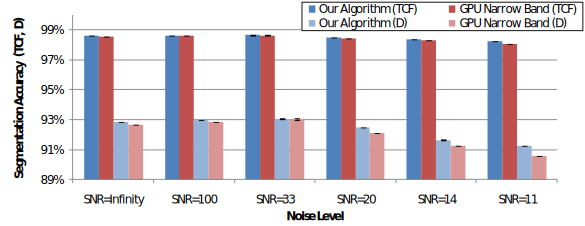
\includegraphics[width=3.0in]{figures/Accuracy.pdf}
\caption{Accuracy of our algorithm and the GPU narrow band algorithm while performing a set of repeated (N=10) white matter segmentations in a $256^3$ head MRI with varying signal-to-noise-ratio (SNR) values. For each segmentation we used a randomly selected seed point and we measured the Dice Coefficient (D) and Total Correct Fraction (TCF). }
\label{fig:8}

\end{figure}
%*******************************************************************************

%*******************************************************************************
% FIGURE 9
\begin{figure*}[t]
\centering
\subfigure[]{
\includegraphics[width=3.0in]{figures/SpeedA1.pdf}
\label{fig:speedA}
}
\subfigure[]{
\includegraphics[width=3.0in]{figures/SpeedB1.pdf}
\label{fig:speedB}
}
\subfigure[]{
\includegraphics[width=3.0in]{figures/SpeedC1.pdf}
\label{fig:speedC}
}
\subfigure[]{
\includegraphics[width=3.0in]{figures/SpeedD1.pdf}
\label{fig:speedD}
}
\caption{Performance of our algorithm and the GPU narrow band algorithm while segmenting the white and grey matter in a $256^3$ head MRI. We measured the size of the active computational domain per iteration (a), computation time per iteration (b), computation time as a function of active computational domain size (c), and the computation time per iteration for each subroutine in our algorithm (d). In (c) we overlay the lines of best fit for each algorithm. Lower is better for all graphs.}
\label{fig:speed}
\end{figure*}
%*******************************************************************************


%We observed that segmenting the white and grey matter in a ${256}^3$ T1w MRI with $SNR=11$ and $INU=40\%$ using the Insight Segmentation and Registration Toolkit took 81 minutes and 4 seconds.

Based on the observed linear relationships between the number of active voxels per iteration and the computation time per iteration (Figure~\ref{fig:speedC}), we conclude that the computational domain would need to be roughly 12\% active before unconditionally updating every voxel would provide a performance benefit over our algorithm. At first glance it may seem as though the GPU narrow band algorithm would provide a performance benefit over our algorithm after the computational domain is roughly 9\% active. However due to the GPU narrow band algorithm processing data in 2D tiles of size $g^2$, an active computational domain of size $n$ using our algorithm will result in a larger active computational domain of size $q$ where $n\le q\le g^2n$ using the GPU narrow band algorithm. We observed that the computational domain remained less than 2\% active during each iteration of our algorithm in all experiments.

% We note that an adaptive scheme for switching between our algorithm and unconditionally updating every voxel based on the size of the active computational domain requires at least $O(n)$ additional work and $O({{\log }_2 n)\ }$ additional steps per iteration. This is because once the supposed adaptive scheme has switched to unconditionally updating every voxel, the active computational domain must be reinitialized in order to determine if it is sufficiently small to switch back to our sparse algorithm. The computation time for unconditionally updating every voxel and explicitly reinitializing the active computational domain during each iteration is shown in Figure~\ref{fig:9}(b). Noting this additional cost we concluded that the computational domain would need to be roughly 14\% active before unconditionally updating every voxel would provide a performance benefit over our algorithm. We observed that the computational domain was less than 2\% active at all times using our algorithm.

We observed that tracking the active computational domain using our algorithm accounted for 77\% of the total computation time and updating the level set field accounted for the remaining 23\% of the total computation time (Figure~\ref{fig:speedD}). We conclude that although most of our computation time goes into tracking the active computational domain, we leverage this cost to avoid the bigger downstream cost of unconditionally updating the entire level set field.


%*******************************************************************************
% FIGURE 10
%\begin{figure}[t]
%\centering
%\includegraphics[width=3.0in]{res/fig10.png}
%\caption{Per component performance of our algorithm while segmenting the white and grey matter in a $256^3$ MRI with a signal-to-noise ratio of 11. Lower is better. }
%\label{fig:10}
%\end{figure}
%*******************************************************************************


%-------------------------------------------------------------------------
\section{Conclusions}
\label{sec:conclusions}

We have presented a new GPU level set segmentation algorithm with immediate applications in computer vision and medical imaging. Our algorithm is the first and only GPU level set segmentation algorithm to be presented in the literature with linear work-complexity and logarithmic step-complexity. Moreover our algorithm makes use of a novel condition on the temporal derivatives of the level set field to limit the active computational domain to the minimal set of changing elements. These innovations improve computational efficiency without affecting segmentation accuracy and create new possibilities for clinical application where speed and interactivity are critical.

% In future we plan to perform a detailed bottleneck analysis to learn more about the relationships between computation and communication inherent in our algorithm and the GPU narrow band algorithm. We also plan to investigate strategies for further improving the cache coherence of our sparse active computational domain. Finally we plan to investigate how our algorithm can be extended to higher-order space and time discretization schemes involving bigger local neighborhoods.

\section*{Acknowledgments}
We thank the anonymous reviewers for their valuable comments and suggestions. This research was supported by the iCORE/Calgary Scientific Inc. Industrial Research Chair in Medical Imaging Informatics, Alberta Innovates -- Health Solutions, the Alberta Heritage Foundation for Medical Research Endowment Fund, the iCORE/Foundation CMG Industrial Research Chair in Scalable Reservoir Visualization, and the Discovery Grants Program from the Natural Sciences and Engineering Research Council of Canada.

%-------------------------------------------------------------------------
\bibliographystyle{eg-alpha}
\bibliography{main}


%-------------------------------------------------------------------------
%\newpage




%-------------------------------------------------------------------------
\appendix
\section{Derivation of the Active Set Condition $\varsigma_{2}$}
\label{app:1}

We define the set of all user-specified parameters to the speed function as $H$ and the user-specified image as $I$. We define $\eta \left({\mathbf x}\right)=\{{\mathbf x},{{\mathbf n}}^{{\mathbf x}}_0,{{\mathbf n}}^{{\mathbf x}}_1,{{\mathbf n}}^{{\mathbf x}}_2,\ldots ,{{\mathbf n}}^{{\mathbf x}}_k\}$ to be the set of coordinates in the immediate neighborhood of some voxel ${\mathbf x}$. We define the set of all of level set field values in the immediate neighborhood of ${\mathbf x}$ at time $t$ as $\Phi \left({\mathbf x},t\right)=\{\phi\left({\mathbf x},t\right),\phi\left({{\mathbf n}}^{{\mathbf x}}_0,t\right),\phi\left({{\mathbf n}}^{{\mathbf x}}_1,t\right),{\phi({\mathbf n}}^{{\mathbf x}}_2,t),\ldots ,{\phi({\mathbf n}}^{{\mathbf x}}_k,t)\}$. We assume that the speed function $F({\mathbf x},t)$ is a function of the level set values around ${\mathbf x}$ during the previous iteration $\Phi \left({\mathbf x},t-\Delta t\right)$, the image $I$, and the set of user-specified parameters $H$. We assume without loss of generality that $\Delta t\ne 0$.

We want to prove that ${\forall }_{{\mathbf n}\in \eta \left({\mathbf x}\right)}:\phi\left({\mathbf n},t-\Delta t\right)=\phi({\mathbf n},t-2\Delta t)$ implies $\phi\left({\mathbf x},t\right)=\phi\left({\mathbf x},t-\Delta t\right)$. If this claim is true, it means that we can exclude $\mathbf{x}$ from our active set at time $t$ if ${\forall }_{{\mathbf n}\in \eta \left({\mathbf x}\right)}:\phi\left({\mathbf n},t-\Delta t\right)=\phi({\mathbf n},t-2\Delta t)$. We begin by proving a useful lemma.

\begin{lem}
$\Phi \left({\mathbf x},t-\Delta t\right)=\Phi \left({\mathbf x},t-2\Delta t\right)$ implies $F\left({\mathbf x},t\right)=F\left({\mathbf x},t-\Delta t\right)$.
\label{lem:1}
\end{lem}

\begin{pro}
We assume $\Phi \left({\mathbf x},t-\Delta t\right)=\Phi \left({\mathbf x},t-2\Delta t\right)$. By definition $F\left({\mathbf x},t\right)=f(\Phi \left({\mathbf x},t-\Delta t\right),I,H)$ for some function $f$. Therefore we get $F\left({\mathbf x},t-\Delta t\right)=f\left(\Phi \left({\mathbf x},t-2\Delta t\right),I,H\right)=f\left(\Phi \left({\mathbf x},t-\Delta t\right),I,H\right)=F\left({\mathbf x},t\right)$. $\qed$
\end{pro}

Now we move onto our central proof.

\begin{cla}
${\forall }_{{\mathbf n}\in \eta \left({\mathbf x}\right)}:\phi\left({\mathbf n},t-\Delta t\right)=\phi({\mathbf n},t-2\Delta t)$ implies $\phi\left({\mathbf x},t\right)=\phi\left({\mathbf x},t-\Delta t\right)$.
\end{cla}

\begin{pro}
We prove by contradiction. We assume that ${\forall }_{{\mathbf n}\in \eta \left({\mathbf x}\right)}:\phi\left({\mathbf n},t-\Delta t\right)=\phi({\mathbf n},t-2\Delta t)$.
From this expression and the definition of $\Phi$ we get $\Phi \left({\mathbf x},t-\Delta t\right)=\Phi \left({\mathbf x},t-2\Delta t\right)$. From Lemma~\ref{lem:1} we get $F\left({\mathbf x},t\right)=F\left({\mathbf x},t-\Delta t\right)$. From the definition of $\nabla \phi$ we get $\nabla \phi\left({\mathbf x},t - \Delta t\right) = \nabla \phi\left({\mathbf x},t - 2 \Delta t\right)$.

\medskip

We assume for the sake of contradiction that $\phi\left({\mathbf x},t\right)\ne \phi\left({\mathbf x},t-\Delta t\right)$. Substituting this inequality into Equation~\ref{eq:1} we get $\phi\left({\mathbf x},t\right)-\phi\left({\mathbf x},t-\Delta t\right)=\Delta tF\left({\mathbf x},t\right)\left|\nabla \phi\left({\mathbf x},t-\Delta t\right)\right|\ne 0$. From the zero product rule we get $F\left({\mathbf x},t\right)\ne 0$ and $\left|\nabla \phi\left({\mathbf x},t-\Delta t\right)\right|\ne 0$.

\medskip

From our initial assumption that ${\forall }_{{\mathbf n}\in \eta \left({\mathbf x}\right)}:\phi\left({\mathbf n},t-\Delta t\right)=\phi({\mathbf n},t-2\Delta t)$, and since ${\mathbf x}\in \eta \left({\mathbf x}\right)$, we get $\phi\left({\mathbf x},t-\Delta t\right)=\phi({\mathbf x},t-2\Delta t)$. Substituting the right hand side of this expression into Equation~\ref{eq:1} we get $\phi\left({\mathbf x},t-\Delta t\right)=\phi\left({\mathbf x},t-\Delta t\right)+\Delta tF\left({\mathbf x},t-\Delta t\right)\left|\nabla \phi\left({\mathbf x},t-2\Delta t\right)\right|$, or equivalently $\Delta tF\left({\mathbf x},t-\Delta t\right)\left|\nabla \phi\left({\mathbf x},t-2\Delta t\right)\right|=0$. From this expression and the zero product rule we get either $F\left({\mathbf x},t-\Delta t\right)=0$ or $\left|\nabla \phi\left({\mathbf x},t-2\Delta t\right)\right|=0$.

\medskip

We assume for the moment that $F\left({\mathbf x},t-\Delta t\right)=0$. Since $F\left({\mathbf x},t\right)=F\left({\mathbf x},t-\Delta t\right)$ we get $F\left({\mathbf x},t\right)=0$ which leads to a contradiction. Now we assume for the moment that $\left|\nabla \phi\left({\mathbf x},t-2\Delta t\right)\right|=0$. From this expression, and since $\nabla \phi\left({\mathbf x},t - \Delta t\right) = \nabla \phi\left({\mathbf x},t - 2 \Delta t\right)$, we get $\left|\nabla \phi\left({\mathbf x},t-\Delta t\right)\right|=0$ which also leads to a contradiction. Therefore $\phi\left({\mathbf x},t\right)=\phi\left({\mathbf x},t-\Delta t\right)$. \qed

\end{pro}

%-------------------------------------------------------------------------
%\section{Proof that our Parallel Algorithm is Work-Efficient and Step-Efficient}
%\label{app:2}

%We prove that our parallel algorithm is both work-efficient and step-efficient by considering each of its subroutines individually. We define $n$ as the size of the active computational domain and $p$ as the size of the entire level set field.

%Listing~\ref{pseudo:1} requires one pass over the entire computational domain and therefore has $O(p)$ work-complexity and $O(1)$ step-complexity.

%The \textbf{for all} loop in Listing~\ref{pseudo:2} requires one pass over the entire computational domain and therefore has $O(p)$ work-complexity and $O(1)$ step-complexity. The call to \textbf{compact} in Listing~\ref{pseudo:2} has $O(p)$ work-complexity and $O({\log}_2 p)$ step-complexity~\cite{Harris-2007,Sengupta-2007,Sengupta-2008}.

%Listing~\ref{pseudo:3} and Listing~\ref{pseudo:4} each require one pass over the active computational domain and therefore each has $O(n)$ work-complexity and $O(1)$ step-complexity.

%Listing~\ref{pseudo:5} requires seven passes over the active computational domain, not including the call to \textbf{compact}, and therefore has $O(n)$ work-complexity and $O(1)$ step-complexity. The call to \textbf{compact} in Listing~\ref{pseudo:5} has $O(n)$ work-complexity and $O({\log}_2 n)$ step-complexity~\cite{Harris-2007,Sengupta-2007,Sengupta-2008}. After Listing~\ref{pseudo:5}, our algorithm must clear $B^{\mathbf{e}}_{0 \ldots n}$ for all offset vectors $\mathbf{e} \in E$. Clearing these buffers has $O(n)$ work-complexity and $O(1)$ step-complexity.

%We conclude that our algorithm has $O(p)$ work-complexity and $O({\log}_2 p)$ step-complexity during initialization. After initialization our algorithm has $O(n)$ work-complexity and $O({\log}_2 n)$ step-complexity. $\qed$

\end{document}
